\chapter{Suporte Tecnológico}
\section{Cloudstack}
Em um modelo simplificado, o cloudstack é composto de uma máquina de gerenciamento e dos recursos a serem gerenciados. Tais recursos compreende: faixa de endereços \textit{IP}, dispositivos \textit{storage},servidores e \textit{VLAN'S}. Para implementação em uma configuração mínima, pode se utilizar uma máquina dedicada apenas para a interface de gerenciamento, mantendo o servidor físico apenas com o \textit{hypervisor}, ou utilizar o servidor físico executando a interface de gerenciamento e o \textit{hypervisor} simultaneamente. 

\begin{figure}[!htb]
\centering
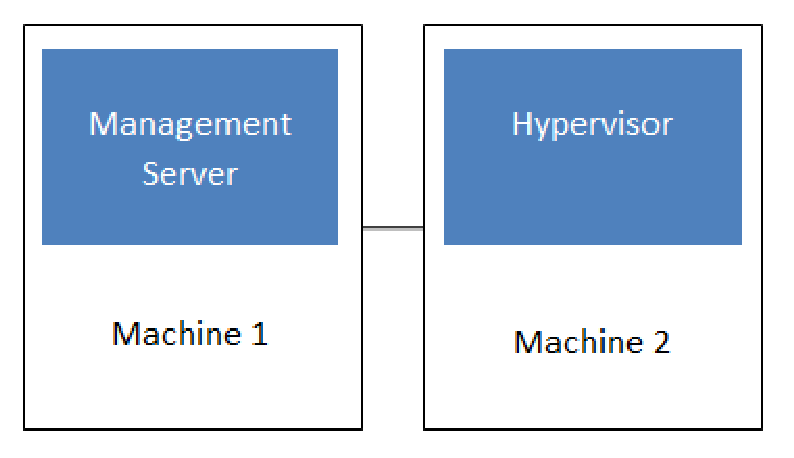
\includegraphics [keepaspectratio=true,scale=0.60]{figuras/cloudstack_minimal.eps}
\caption{Visão simplificada de uma instalação mínima do cloudstack}
\cite{cloudstack}.
\label{cloudstatck_minimal}
\end{figure}

Em modelo mais complexo, o cloudstack apresenta seu pontencial de disponibilidade escalabilidade e gerenciamento. Proporcionando uma modelagem de várias
infraestrutura em nuvens em uma determinada região. Desse modo o cloudstack possui os seguintes níveis de abstrações \cite{shape}:

\begin{itemize}
\item \textbf{Regiões:} são a primeira e maior unidade de escala de uma implementação de uma cloud com CloudStack. Uma Região consiste em multiplas Zonas de Disponibilidade, a segunda maior unidade de escala.
\item \textbf{Zonas: } Tipicamente existe apenas uma Zona por Data Center e cada Zona contem PODs, Hosts e Storage.
\item \textbf{Pods: } PODs tem propriedades lógicas e físicas com componentes como endereçamento IP e algoritmo de alocação de Máquinas Virutais sendo influenciados por PODs dentro de uma Zona.
\item \textbf{Clusters: } São simples grupos de servidores homogêneos combinados com um Storage Primário. Cada Cluster utiliza um mesmo tipo de hypervisor mas em uma Zona pode ceoxistir combinações de todos os hypervisores suportados. Cada Cluster utiliza um mesmo tipo de hypervisor mas em uma Zona pode ceoxistir combinações de todos os hypervisores suportados.
\item \textbf{Hosts: } Responsável por disponibilizar a camada de computação real em que Máquinas Virtuais são executadas.
\item \textbf{Storage Primário: }  onde os discos das Máquinas Virtuais residem e pode ser utilizado o disco local de um Host ou um storage compartilhado como NFS, iSCSI, Fiber Channel, etc.
\item \textbf{Storage Secundário:} onde é armazenado os Templates de Máquinas Virtuais, arquivos ISO e Snapshots e é utilizado o protocolo NFS para este Storage
\end{itemize}


\begin{figure}[!htb]
\centering
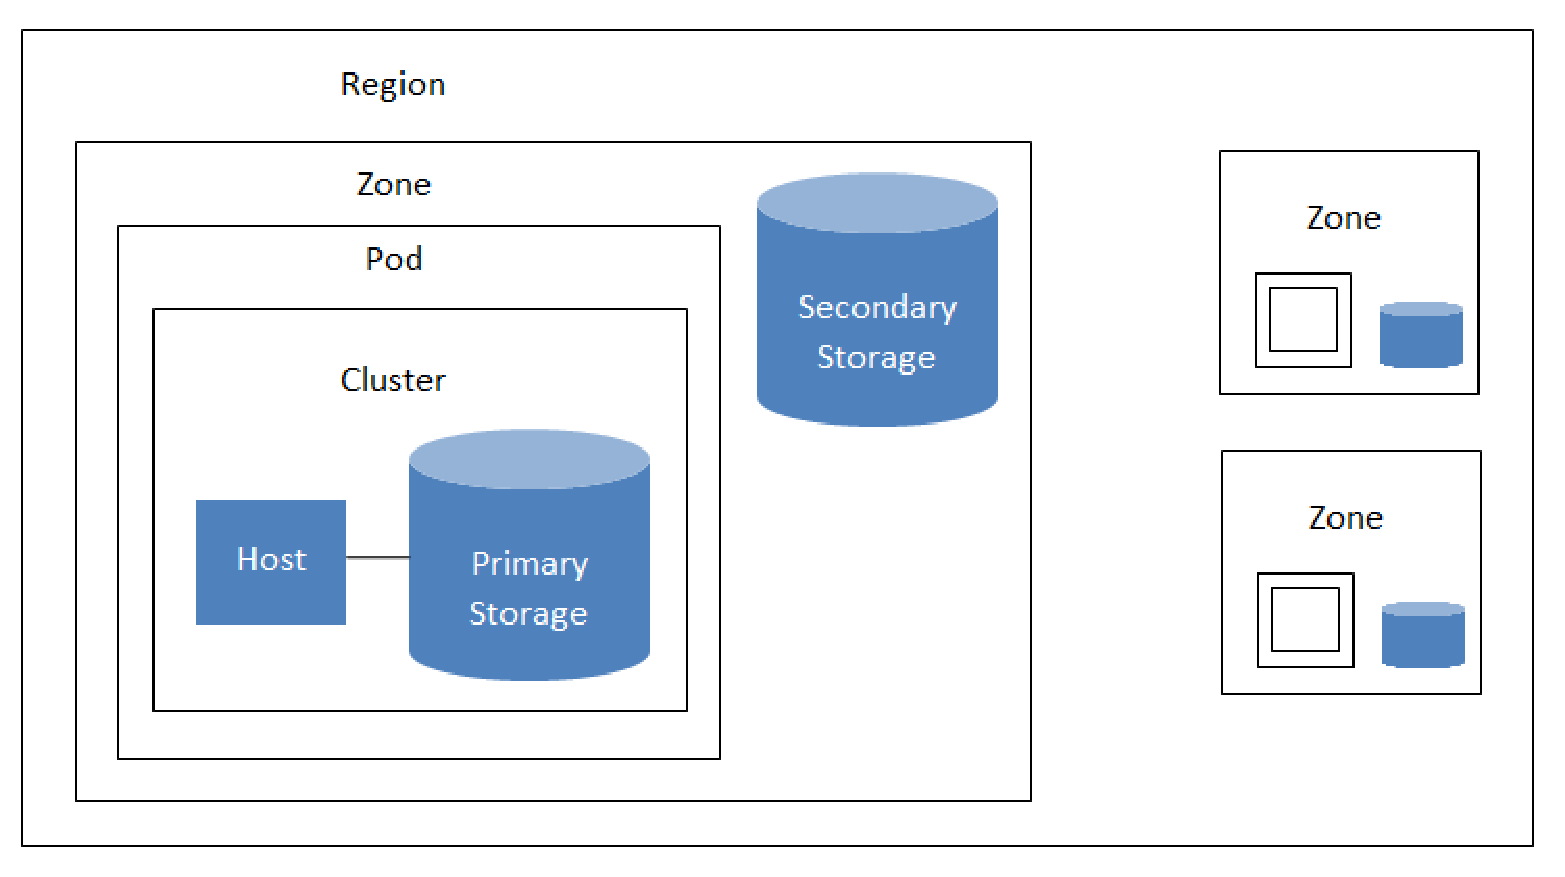
\includegraphics [keepaspectratio=true,scale=0.60]{figuras/cloudstack_structure.eps}
\caption{Visão geral da infraestrutura do Cloudstack}
\cite{cloudstack}.
\label{diagramacloudstack}
\end{figure}

\section{OpenNebula}
O \textit{OpenNebula}, assim como o \textit{cloudstack}, é uma ferramenta de código aberto que emergiu como um projeto de pesquisa em 2005 tendo seu primeiro lançamento público em março de 2008. Oferece uma solução simples mas repleta de funcionalidades para construir e gerenciar nuvens corporativas e \textit{data centers} virtuais. Alem disso, combina tecnologias de virtualização existentes com funcionalides avançadas para fornecimento automático e elasticidade, seguindo uma abordagem \textit{bottom-up}, guiado pelas reais necessidades de adminstradores de sistemas e \textit{devops}\cite{opennebula}.

Em uma configuração mínima  arquitetura do \textit{OpenNebula} é composta por três componentes: \textit{hosts}, \textit{datastores} e \textit{front-end}. O \textit{front-end} é a máquina responsável por disponinbilizar a interface de gerenciamento. Através da rede, monitora os \textit{hosts} e máquinas virtuais, bem como inicia operações relacionadas com máquinas virtuais e \textit{datastores}. Os \textit{hosts} ou \textit{worker nodes} são as máquinas físicas responsáveis pelos recursos físicos essenciais para a criação de máquinas virtuais, é nesta máquina onde o \textit{hypervisor} será instalado. Por fim, os \textit{datastore} é o \textit{storage} utilizado como repositório de imagens e para manter os discos das máquinas virtuais, em execução. Não precisa ser necessariamente um storage dedicado, podendo ser uma máquina física com mais capacidade de disco ou até mesmo sendo um dos próprios \textit{hosts}.  


\begin{figure}[!htb]
\centering
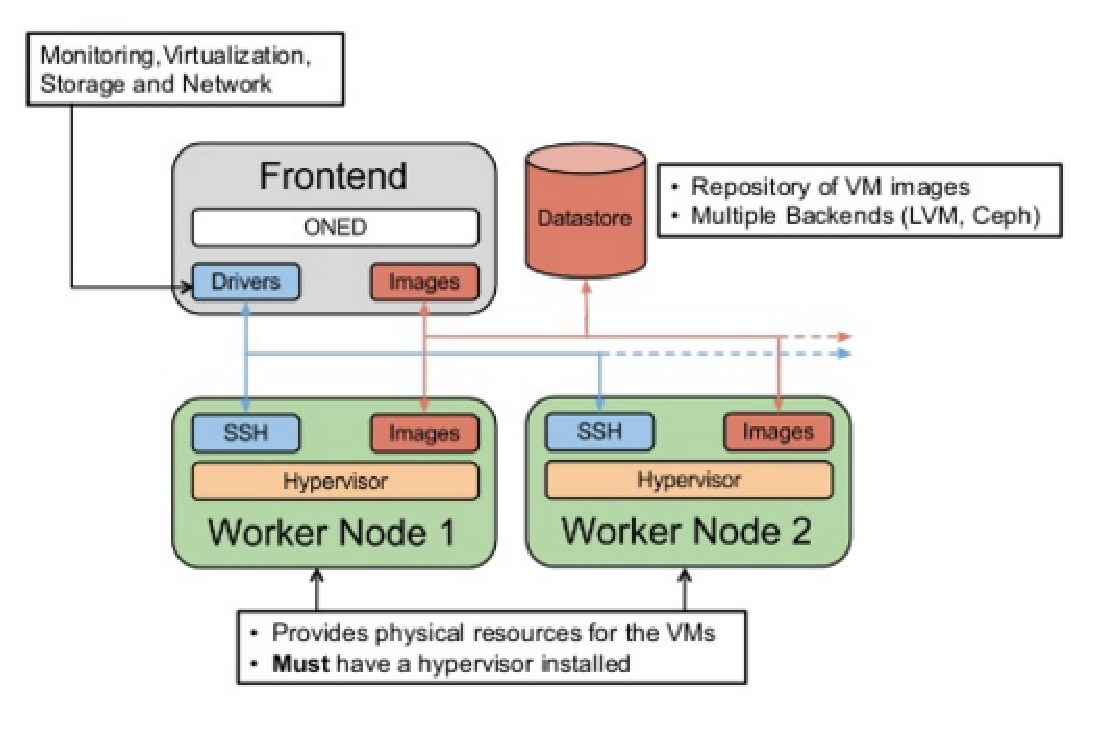
\includegraphics [keepaspectratio=true,scale=0.70]{figuras/opennebula_instalation.eps}
\caption{Visão geral da infraestrutura do OpenNebula}
\cite{opennebula}.
\label{diagramaopennebula}
\end{figure}

O \textit{System Datastore} é uma abstração do OpenNebula ao qual é responsável por manter os discos das máquinas virtuais em execução. Possui três tipos\cite{opennebula}:

\begin{itemize}
\item \textit{\textbf{shared}} - O \textit{System Datastore} é compartilhado entre todos os outros hots usando \textit{NFS}, por exemplo.
\item \textit{\textbf{vmfs}} - Necessário quando o \textit{hypervisor} utilizado é o \textit{VMware}. Uma versão da opção \textit{shared} voltada para o sistemas de arquivos do \textit{VMware}.
\item \textit{\textbf{ssh}} - Nesse caso, cada host possui seu próprio \textit{System Datastore}.
\end{itemize}

\begin{figure}[!htb]
\centering
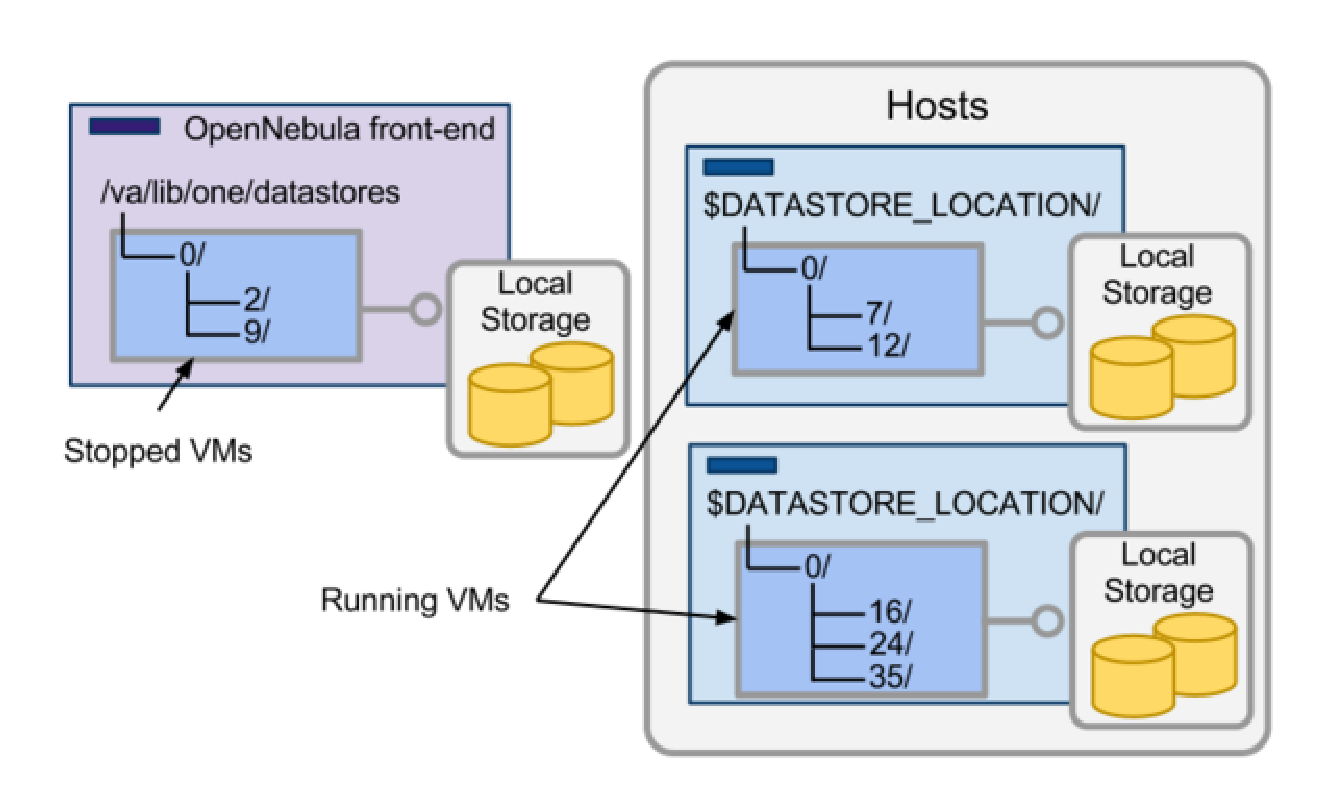
\includegraphics [keepaspectratio=true,scale=0.60]{figuras/ssh_datastore.eps}
\caption{Funcionamento do \textit{System Datastore} na configuração \textit{SSH}.}
\cite{opennebula}.
\label{ssh_datastore}
\end{figure}

\begin{figure}[!htb]
\centering
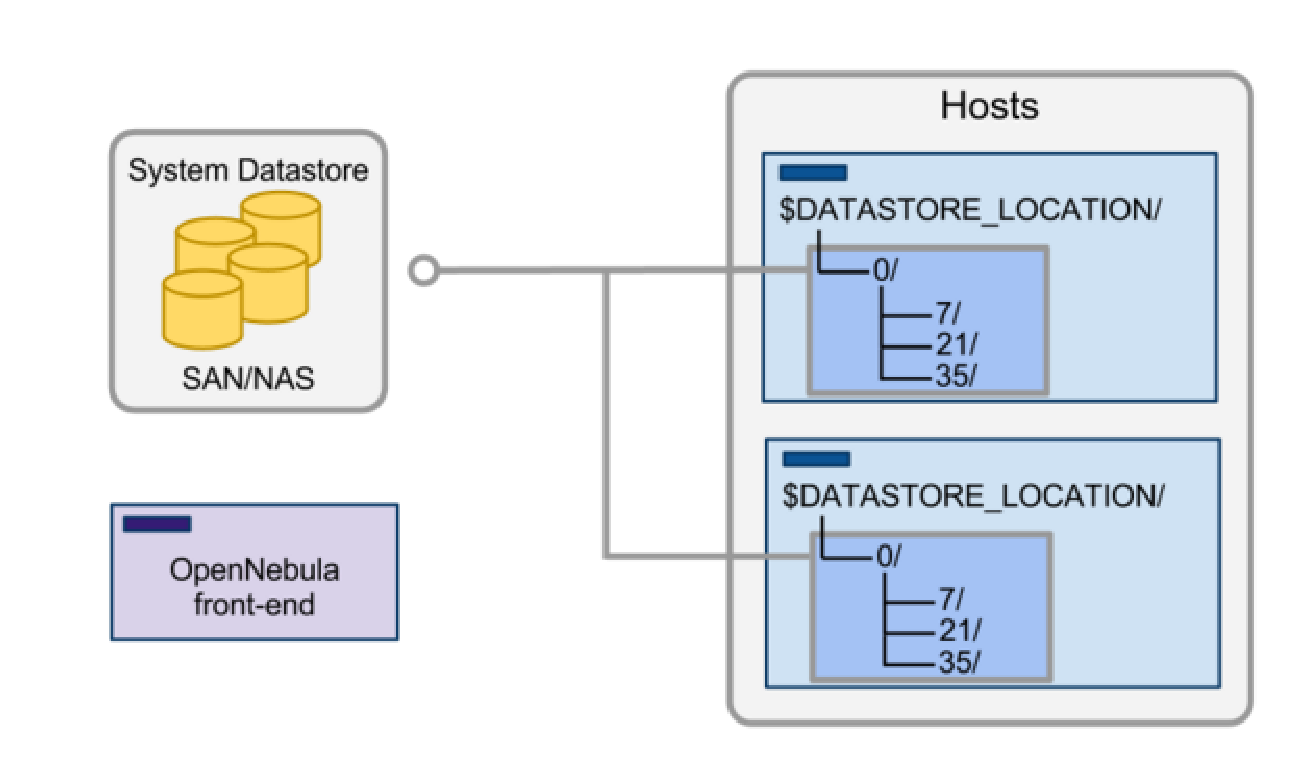
\includegraphics [keepaspectratio=true,scale=0.60]{figuras/shared_datastore.eps}
\caption{Funcionamento do \textit{System Datastore} na configuração \textit{shared}. }
\cite{opennebula}.
\label{shared_datastore}
\end{figure}

O \textit{OpenNebula} possui modelos de implementação tanto para nuvens privadas mais simplifcadas quanto para ambientes de infraestrutura mais complexos. Desse modo, para poucos servidores a implementação do \textit{OpenNebula} é efetuada sem necessidade de ter que se preocupar elementos voltadas para uma infraestrutura maior, que no caso do OpenNebula é chamada de \textit{Federação}. Entretanto, para locais ou empresas que possuem múltiplos \textit{data centers}, que por sua vez, possui vários \textit{clusters} de servidores, o opennebula prover funcionalidades que colaboram para que vários data centers separados regionalmente possam ser gerenciados a partir de uma interface em nuvem com acesso externo. 

Cada instância do opennebula é denominada de zona, desse modo em uma infraestrutura com múltiplas zonas pode ser configuradas como uma Federação. Assim, tem-se um compartilhamento da base de dados entre as zonas(Usuários, grupos). Nessa configuração, uma das zonas tem o papel de \textit{master}, ao qual é o responsável por escrever as informações na base dados, mantendo assim a consistência nos dados\cite{opennebula}.

\begin{figure}[!htb]
\centering
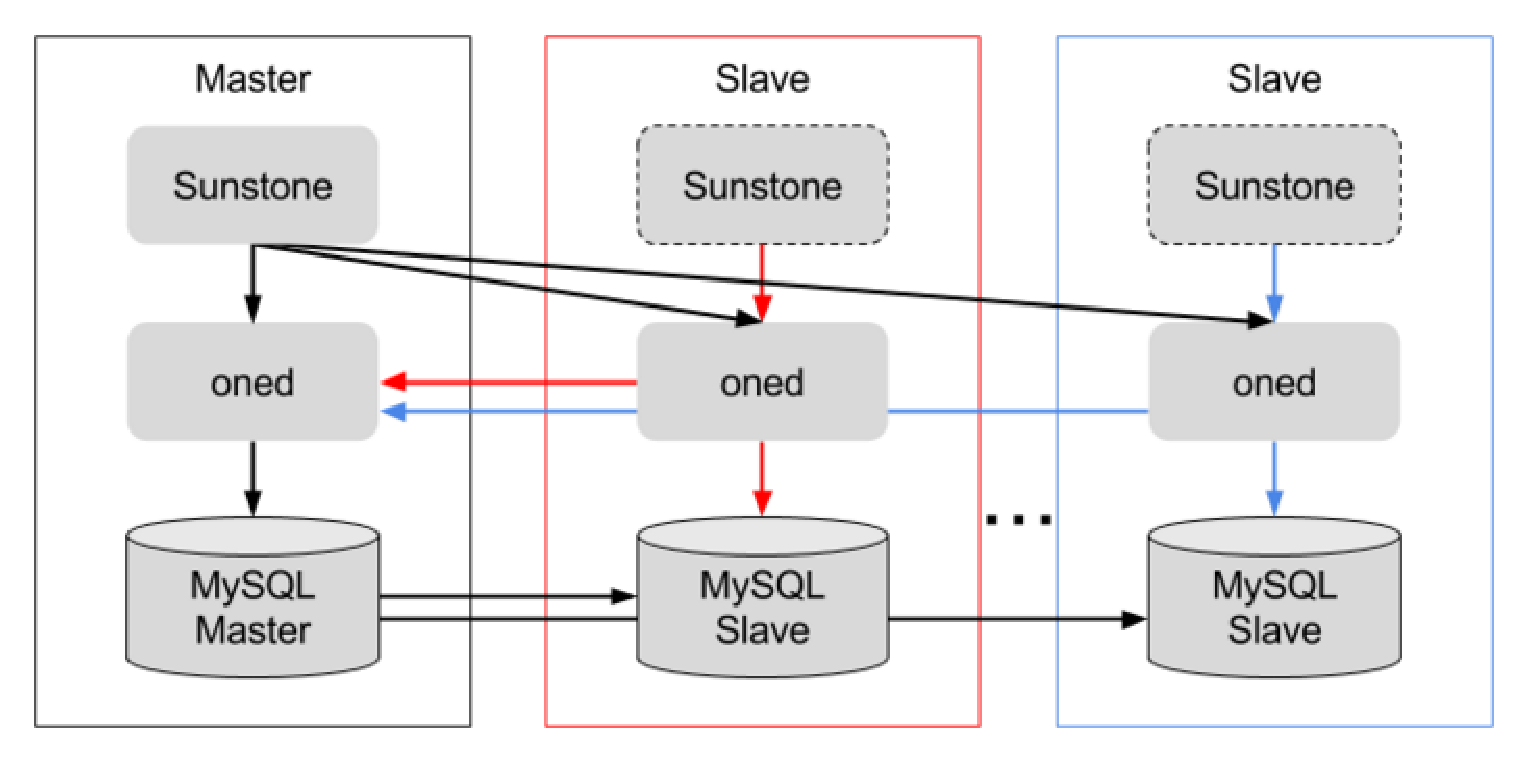
\includegraphics [keepaspectratio=true,scale=0.50]{figuras/opennebula_zone.eps}
\caption{Arquitetura de implantação por zonas}
\cite{opennebula}.
\label{opennebulafederation}
\end{figure}

\section{Comparativo entre as ferramentas de Plataforma em nuvem}

Nesta seção é apresentado um breve comparativo entre as ferramentas \textit{OpenNebula} e \textit{Cloudstack} baseado no trabalho de \citeonline{salam}. De acordo com \citeonline{salam}, de maneira geral tanto cloudstack quanto o opennebula possuem funcionlidades que proporcionam um excelente \textit{feedback} com relação ao provimento de plataformas em nuvem. O \textit{OpenNebula} tem como pontos fortes a flexibilidade e escalabilidade o que proporciona um certo dinanismo na adição de novos recursos. Já o \textit{Cloudstack} provê uma API que proporcina facilidades no que diz respeito a integração de outras ferramentas, possibilitando bons mecanismos para configuração da plataforma como um todo \cite{salam}. Entretanto, dos fatores apresentado na tabela x, a robustez contra erros foi decisivo para escolha em favor do OpenNebula, dado que , como será relatado na seção tal, o Cloudstack mostrou-se bastante instável e intolerantes a erros.

